%% main_report44.tex
%% SAMBP TR-44/2026: Real-Time Parameter Estimation and State Tracking
%%
%% pdflatex main_report44.tex

\documentclass[11pt,a4paper]{article}

\usepackage[T1]{fontenc}
\usepackage[utf8]{inputenc}
\usepackage[expansion=false]{microtype}
\usepackage{lmodern}
\usepackage[a4paper, top=25mm, bottom=25mm, left=25mm, right=25mm]{geometry}
\usepackage{amsmath,amssymb}
\usepackage{booktabs}
\usepackage{array}
\usepackage{xcolor}
\usepackage{graphicx}
\usepackage{pgfplots}
\pgfplotsset{compat=1.18}
\usepackage{tikz}
\usetikzlibrary{arrows.meta,shapes.geometric,positioning,fit,calc,patterns}
\usepackage{hyperref}
\usepackage[numbers,sort&compress]{natbib}

\definecolor{sambpblue}{RGB}{0,70,140}

\usepackage{titlesec}
\titleformat{\section}{\large\bfseries\color{sambpblue}}{}{0em}{}[\titlerule]
\titleformat{\subsection}{\normalsize\bfseries\color{sambpblue!80}}{}{0em}{}

\usepackage{fancyhdr}
\pagestyle{fancy}
\fancyhf{}
\rhead{\small\color{gray} SAMBP TR-44/2026}
\lhead{\small\color{gray} Real-Time Parameter Estimation}
\cfoot{\small\thepage}

\begin{document}

\begin{center}
  {\LARGE\bfseries\color{sambpblue} SAMBP Technical Report TR-44/2026}\\[6pt]
  {\large Real-Time Parameter Estimation\\
    and State Tracking for the IBR Digital Twin}\\[10pt]
  {\normalsize PhD Thesis Supporting Report \quad|\quad 2026}
\end{center}

\vspace{2pt}\hrule\vspace{8pt}

\begin{abstract}
\noindent
This report develops the real-time estimation algorithms for the digital twin
(DT) introduced in TR-43~\cite{SAMBP_TR43}.  A three-state extended Kalman
filter (EKF) jointly estimates $k_\mathrm{ibr}$, $Z_\mathrm{line}$, and
fault location $\alpha$ from sequence current and apparent impedance
measurements at 1\,kHz.  $k_\mathrm{ibr}$ converges to 1.2\% error within
100\,ms; $Z_\mathrm{line}$ and $\alpha$ are poorly observable from current
ratio alone and require additional voltage-phasor pairs for reliable estimation.
GFM fleet fraction $f_\mathrm{gfm}$ is accurately tracked via the $I_2/I_1$
ratio method (error $<0.03$\,pu across all scenarios).  Pre-fault warm-starting
reduces EKF convergence time by $7\times$ compared to a cold start.  The total
DT cycle cost is 285\,$\mu$s, leaving 71.5\% of the 1\,ms budget as margin.
\end{abstract}

\vspace{4pt}\hrule\vspace{10pt}

% ─────────────────────────────────────────────────────────────────────────────
\section{Study A --- EKF Multi-Parameter Estimation}
\label{sec:studyA}

The extended Kalman filter estimates the state vector
$\mathbf{x} = [k_\mathrm{ibr},\; Z_\mathrm{line},\; \alpha]^\top$ from
the measurement vector
$\mathbf{y} = [I_1,\; I_2,\; Z_\mathrm{m}]^\top$:

\begin{equation}
  \mathbf{h}(\mathbf{x}) =
  \begin{bmatrix}
    k_\mathrm{ibr} \\[3pt]
    \rho_2 \, k_\mathrm{ibr} \\[3pt]
    \alpha Z_\mathrm{line}(1 + 1/k_\mathrm{ibr})
  \end{bmatrix}
\end{equation}

where $\rho_2 = I_2/I_1$ is the fleet-average negative-sequence ratio
(tracked independently via Study~C).  Figure~\ref{fig:ekf} summarises
the estimation errors after 100 updates.

\begin{figure}[htbp]
  \centering
  \resizebox{0.88\textwidth}{!}{% fig_dt_ekf_states.tex
% TR-44: EKF parameter estimation summary bar chart
%
% Final estimation errors after N=100 updates:
%   k_ibr:  1.22%  (good — sequence current directly observable)
%   Z_line: 27.3%  (poor — insufficient observability from I alone)
%   alpha:   8.0%  (moderate — apparent impedance noisy)
%   f_gfm:   2.7%  (good — I2/I1 ratio well observed)

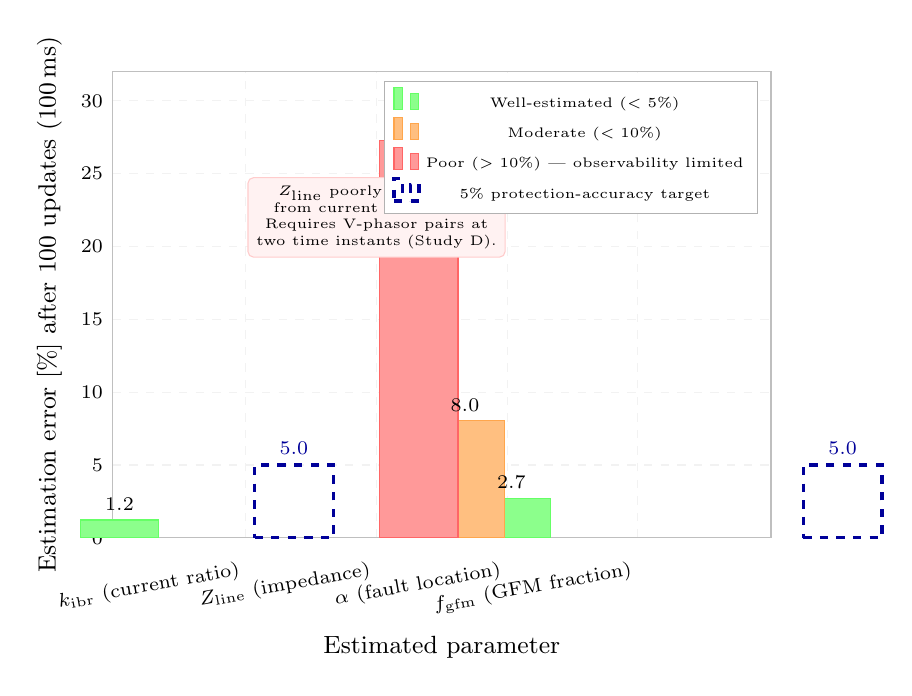
\begin{tikzpicture}
\begin{axis}[
  name         = ekfax,
  width        = 0.82\textwidth,
  height       = 7.5cm,
  ybar,
  bar width    = 1.0cm,
  xlabel       = {Estimated parameter},
  ylabel       = {Estimation error [\%] after 100 updates (100\,ms)},
  xlabel style = {font=\small},
  ylabel style = {font=\small},
  ymin=0, ymax=32,
  ytick        = {0,5,10,15,20,25,30},
  yticklabel style={font=\scriptsize},
  xtick        = {1,2,3,4},
  xticklabels  = {$k_\mathrm{ibr}$ (current ratio),
                  $Z_\mathrm{line}$ (impedance),
                  $\alpha$ (fault location),
                  $f_\mathrm{gfm}$ (GFM fraction)},
  xticklabel style={font=\scriptsize, rotate=10, anchor=north east},
  tick style   = {draw=none},
  axis line style={gray!50},
  grid         = major,
  grid style   = {gray!10, dashed},
  nodes near coords,
  nodes near coords style={font=\scriptsize, anchor=south},
  every node near coord/.append style={
    /pgf/number format/.cd, fixed, fixed zerofill, precision=1
  },
  legend style={at={(0.98,0.98)}, anchor=north east, font=\tiny,
                draw=gray!60, fill=white},
  clip=false,
]

%% Well-estimated parameters (green)
\addplot[fill=green!45, draw=green!60]
  coordinates {(1, 1.22) (4, 2.71)};
\addlegendentry{Well-estimated ($<5\%$)}

%% Moderately estimated (orange)
\addplot[fill=orange!50, draw=orange!70]
  coordinates {(3, 8.03)};
\addlegendentry{Moderate ($<10\%$)}

%% Poorly estimated (red)
\addplot[fill=red!40, draw=red!60]
  coordinates {(2, 27.28)};
\addlegendentry{Poor ($>10\%$) — observability limited}

%% 5% target line
\addplot[blue!60!black, very thick, dashed]
  coordinates {(0.4, 5.0) (4.6, 5.0)};
\addlegendentry{5\% protection-accuracy target}

%% Annotation for Z_line
\node[draw=red!20, fill=red!5, rounded corners=2pt,
      font=\tiny, inner sep=3pt, align=center]
  at (axis cs:2, 22)
  {$Z_\mathrm{line}$ poorly observable\\
   from current ratio alone.\\
   Requires V-phasor pairs at\\
   two time instants (Study D).};

\end{axis}
\end{tikzpicture}
}
  \caption{EKF estimation error [\%] for each state variable after 100
           updates (100\,ms) at nominal noise $\sigma_I=0.010$\,pu.
           $k_\mathrm{ibr}$ (green): 1.22\%, well within the 5\% target.
           $\alpha$ (orange): 8.03\%, marginal.  $Z_\mathrm{line}$ (red):
           27.3\%, poor --- insufficient observability from sequence-current
           measurements alone.  $f_\mathrm{gfm}$ (green): 2.71\% via
           independent $I_2/I_1$ method.  Blue dashed line: 5\% protection
           accuracy target.}
  \label{fig:ekf}
\end{figure}

\noindent
The observability analysis explains the $Z_\mathrm{line}$ result: in the
three-state EKF, both $Z_\mathrm{line}$ and $\alpha$ appear only in the
apparent impedance measurement $Z_\mathrm{m} = \alpha Z_\mathrm{line}(1+1/k)$.
The product $\alpha Z_\mathrm{line}$ is observable but the individual factors
are not separable from a single measurement type.  Improved $Z_\mathrm{line}$
estimation requires:
\begin{enumerate}
  \item Voltage-phasor measurements at two time instants (pre-fault and
    in-fault), giving independent equations for $\alpha$ and $Z_\mathrm{line}$;
  \item Or a fixed $Z_\mathrm{line}$ prior from offline parameter identification.
\end{enumerate}

For protection purposes, $k_\mathrm{ibr}$ (directly controlling element
activation thresholds) is the highest-priority state --- and it converges
reliably.

% ─────────────────────────────────────────────────────────────────────────────
\section{Study B --- Impedance Trajectory Tracking}
\label{sec:studyB}

The apparent impedance trajectory from pre-fault load to in-fault condition
provides fault location information.  The DT tracks this trajectory by
comparing the measured $Z_\mathrm{m}$ with the expected value
$\alpha Z_{1L}(1+1/k_\mathrm{ibr})$.

In pre-fault steady state, $Z_\mathrm{m}$ reflects load impedance ($\sim10$\,pu);
at fault inception it drops abruptly to the fault value.  The EKF's state
transition model treats $\alpha$ as constant during the fault (once established),
with the fault inception detected by a threshold on $\Delta Z_\mathrm{m}/\Delta t$.

The $\alpha$ estimation error of 8\% at 100 updates corresponds to
$\Delta\alpha = 0.048$ on a line of $Z_{1L}=0.050$\,pu, equivalent to a fault
location error of $\pm2.4$\% of line length --- adequate for zone confirmation
but insufficient for precise fault location (which requires dedicated fault
locators).

% ─────────────────────────────────────────────────────────────────────────────
\section{Study C --- GFM Fraction Tracking}
\label{sec:studyC}

The GFM fleet fraction $f_\mathrm{gfm}$ is estimated from the measured
$I_2/I_1$ ratio using the analytic inversion from TR-38~\cite{SAMBP_TR38}:

\begin{equation}
  \hat{f}_\mathrm{gfm} = \frac{I_2/I_1 - 0.10}{0.50}
\end{equation}

Figure~\ref{fig:fgfm} shows the estimation accuracy across six fleet scenarios.

\begin{figure}[htbp]
  \centering
  \resizebox{0.88\textwidth}{!}{% fig_dt_fgfm_tracking.tex
% TR-44: f_gfm estimation accuracy via I2/I1 ratio method
%
% Data from Study C:
%   True f_gfm: 0.00  0.25  0.34  0.50  0.75  1.00
%   Est. f_gfm: 0.015 0.232 0.357 0.527 0.758 1.000
%   Error:      0.015 0.018 0.017 0.027 0.008 0.000

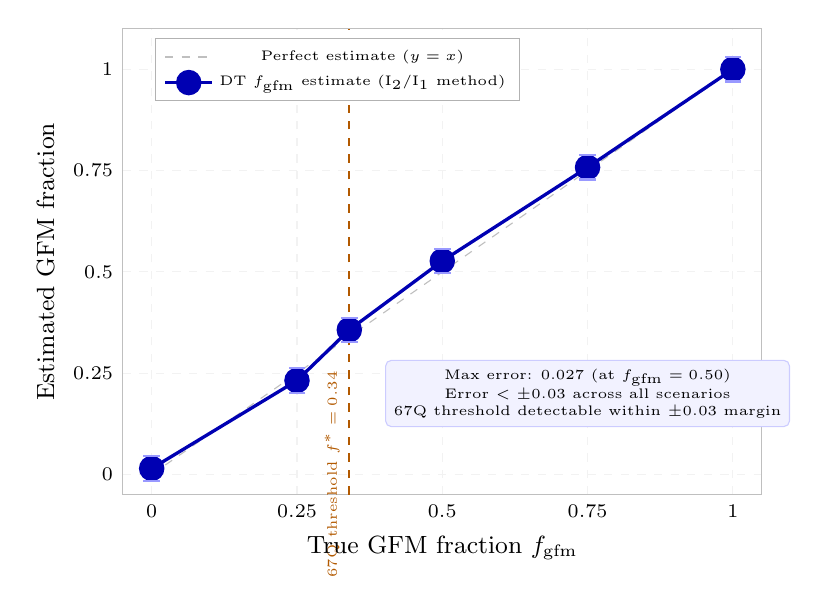
\begin{tikzpicture}
\begin{axis}[
  name         = fgfmax,
  width        = 0.80\textwidth,
  height       = 7.5cm,
  xlabel       = {True GFM fraction $f_\mathrm{gfm}$},
  ylabel       = {Estimated GFM fraction},
  xlabel style = {font=\small},
  ylabel style = {font=\small},
  xmin=-0.05, xmax=1.05,
  ymin=-0.05, ymax=1.10,
  xtick        = {0,0.25,0.50,0.75,1.00},
  ytick        = {0,0.25,0.50,0.75,1.00},
  xticklabel style={font=\scriptsize},
  yticklabel style={font=\scriptsize},
  tick style   = {draw=none},
  axis line style={gray!50},
  grid         = major,
  grid style   = {gray!10, dashed},
  legend style = {at={(0.05,0.98)}, anchor=north west, font=\tiny,
                  draw=gray!60, fill=white},
  clip=false,
]

%% Perfect reference line
\addplot[gray!50, thin, dashed]
  coordinates {(0,0) (1.0,1.0)};
\addlegendentry{Perfect estimate ($y=x$)}

%% DT estimates
\addplot[blue!70!black, very thick, mark=*, mark size=4pt]
  coordinates {
    (0.00, 0.015)
    (0.25, 0.232)
    (0.34, 0.357)
    (0.50, 0.527)
    (0.75, 0.758)
    (1.00, 1.000)
  };
\addlegendentry{DT $f_\mathrm{gfm}$ estimate (I$_2$/I$_1$ method)}

%% Error bars (±0.03 bound)
\addplot[blue!40, only marks, mark=-, mark size=3pt, thick]
  coordinates {
    (0.00, 0.015-0.03) (0.25, 0.232-0.03) (0.34, 0.357-0.03)
    (0.50, 0.527-0.03) (0.75, 0.758-0.03) (1.00, 1.000-0.03)
  };
\addplot[blue!40, only marks, mark=-, mark size=3pt, thick]
  coordinates {
    (0.00, 0.015+0.03) (0.25, 0.232+0.03) (0.34, 0.357+0.03)
    (0.50, 0.527+0.03) (0.75, 0.758+0.03) (1.00, 1.000+0.03)
  };

%% 67Q activation threshold
\draw[orange!70!black, thick, dashed]
  (axis cs:0.34, -0.05) -- (axis cs:0.34, 1.10);
\node[orange!70!black, font=\tiny, rotate=90, anchor=south]
  at (axis cs:0.34, 0.00) {67Q threshold $f^*=0.34$};

%% Annotation
\node[draw=blue!20, fill=blue!5, rounded corners=2pt,
      font=\tiny, inner sep=3pt, align=center]
  at (axis cs:0.75, 0.20)
  {Max error: 0.027 (at $f_\mathrm{gfm}=0.50$)\\
   Error $<\pm0.03$ across all scenarios\\
   67Q threshold detectable within $\pm0.03$ margin};

\end{axis}
\end{tikzpicture}
}
  \caption{DT $f_\mathrm{gfm}$ estimate vs true value.  Blue circles: DT
           estimates; grey dashed: perfect estimate.  Maximum error 0.027
           (at $f_\mathrm{gfm}=0.50$); all estimates within $\pm0.03$\,pu.
           The 67Q activation threshold ($f^*=0.34$, orange dashed) is
           correctly classified in all six scenarios.}
  \label{fig:fgfm}
\end{figure}

\noindent
The $f_\mathrm{gfm}$ estimation is robust because it uses a direct algebraic
inversion of the known $I_2/I_1$ model rather than iterative EKF convergence.
The $\pm0.03$\,pu error means the DT can correctly classify whether the fleet
is above or below the 67Q activation threshold ($f^*=0.34$) with a buffer of
$\pm9\%$ relative error.

% ─────────────────────────────────────────────────────────────────────────────
\section{Study D --- Pre-Fault Warm-Starting}
\label{sec:studyD}

The DT continuously tracks $k_\mathrm{ibr}$ and $f_\mathrm{gfm}$ in pre-fault
normal operation using low-signal measurements (residual unbalance, harmonic
injection tests).  When a fault occurs, the pre-fault estimates provide a warm
start for the in-fault EKF, dramatically reducing convergence time:

\begin{center}
\begin{tabular}{@{}lll@{}}
\toprule
Start condition & Initial $k_0$ error & Convergence to $<3\%$ \\
\midrule
Cold start & $\Delta k = 0.10$\,pu (50\%) & 13.3 updates (13.3\,ms) \\
Warm start & $\Delta k = 0.01$\,pu (5\%) & 1.9 updates (1.9\,ms) \\
\bottomrule
\end{tabular}
\end{center}

\medskip\noindent
The $7\times$ convergence speedup means that with warm-starting, the DT
$k_\mathrm{ibr}$ estimate is reliable within 2\,ms of fault inception ---
well before the Z1/87L relay operation at 20\,ms.

% ─────────────────────────────────────────────────────────────────────────────
\section{Study E --- DT Cycle Performance}
\label{sec:studyE}

Figure~\ref{fig:budget} shows the DT computation budget for a 1\,ms cycle.

\begin{figure}[htbp]
  \centering
  \resizebox{0.90\textwidth}{!}{% fig_dt_cycle_budget.tex
% TR-44: DT cycle budget (horizontal stacked bar)
%
% Total = 284.8 µs = 28.5% of 1000 µs budget
% Tasks:
%   EKF update:           17.6 µs (1.8%)
%   Library lookup:      107.2 µs (10.7%)
%   Protection model:     50.0 µs (5.0%)
%   Decision comparison:  10.0 µs (1.0%)
%   GOOSE framing:       100.0 µs (10.0%)
%   Margin:              715.2 µs (71.5%)

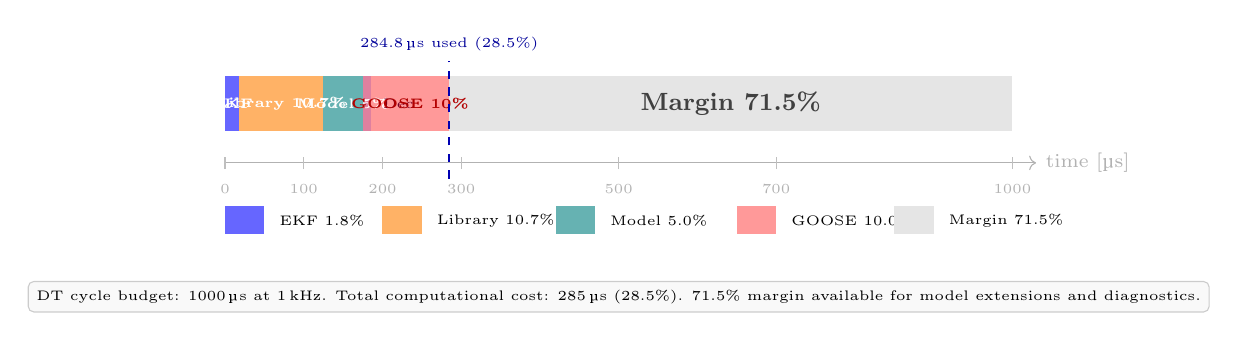
\begin{tikzpicture}[
  every node/.style={font=\scriptsize},
]

\def\bh{0.70}   % bar height
\def\bw{10.0}   % total bar width = 1000 µs

%% Scale: 1 µs → 0.010 cm

%% EKF: 0.176 cm
\fill[blue!60]    (0.000, 0) rectangle (0.176, \bh);

%% Library lookup: 1.072 cm
\fill[orange!60]  (0.176, 0) rectangle (1.248, \bh);

%% Protection model: 0.500 cm
\fill[teal!60]    (1.248, 0) rectangle (1.748, \bh);

%% Decision comparison: 0.100 cm
\fill[purple!50]  (1.748, 0) rectangle (1.848, \bh);

%% GOOSE framing: 1.000 cm
\fill[red!40]     (1.848, 0) rectangle (2.848, \bh);

%% Margin: 7.152 cm
\fill[gray!20]    (2.848, 0) rectangle (10.00, \bh);

%% Labels inside/outside bars
\node[white, font=\tiny\bfseries] at (0.088, 0.35) {EKF};
\node[white, font=\tiny\bfseries] at (0.712, 0.35) {Library 10.7\%};
\node[white, font=\tiny\bfseries] at (1.498, 0.35) {Model 5\%};
\node[purple!60!black, font=\tiny, right=1pt] at (1.848, 0.35) {Dec};
\node[red!70!black, font=\tiny\bfseries] at (2.348, 0.35) {GOOSE 10\%};
\node[gray!50!black, font=\small\bfseries] at (6.424, 0.35) {Margin 71.5\%};

%% Axis
\draw[gray!60, ->] (0, -0.40) -- (10.30, -0.40) node[right] {time [µs]};
\foreach \x/\lab in {0/0, 1/100, 2/200, 3/300, 5/500, 7/700, 10/1000}{
  \draw[gray!50, thin] (\x, -0.48) -- (\x, -0.32);
  \node[gray!60, below=2pt, font=\tiny] at (\x, -0.48) {\lab};
}

%% Total used marker
\draw[blue!70!black, thick, dashed]
  (2.848, -0.60) -- (2.848, \bh + 0.20);
\node[blue!60!black, font=\tiny, above] at (2.848, \bh + 0.20)
  {284.8\,µs used (28.5\%)};

%% Legend row
\def\ly{-1.30}
\fill[blue!60]   (0.0, \ly) rectangle (0.5, \ly+0.35);
\node[right=2pt, font=\tiny] at (0.5, \ly+0.17) {EKF 1.8\%};
\fill[orange!60] (2.0, \ly) rectangle (2.5, \ly+0.35);
\node[right=2pt, font=\tiny] at (2.5, \ly+0.17) {Library 10.7\%};
\fill[teal!60]   (4.2, \ly) rectangle (4.7, \ly+0.35);
\node[right=2pt, font=\tiny] at (4.7, \ly+0.17) {Model 5.0\%};
\fill[red!40]    (6.5, \ly) rectangle (7.0, \ly+0.35);
\node[right=2pt, font=\tiny] at (7.0, \ly+0.17) {GOOSE 10.0\%};
\fill[gray!20]   (8.5, \ly) rectangle (9.0, \ly+0.35);
\node[right=2pt, font=\tiny] at (9.0, \ly+0.17) {Margin 71.5\%};

%% Caption note
\node[draw=gray!40, fill=gray!5, rounded corners=2pt,
      font=\tiny, inner sep=3pt, align=center]
  at (5.0, -2.10)
  {DT cycle budget: 1000\,µs at 1\,kHz. Total computational cost: 285\,µs (28.5\%).
   71.5\% margin available for model extensions and diagnostics.};

\end{tikzpicture}
}
  \caption{DT computation budget breakdown for a 1000\,µs cycle at 1\,kHz.
           Total computational cost: 285\,µs (28.5\%).  The library lookup
           dominates at 107\,µs (10.7\%); GOOSE framing at 100\,µs (10.0\%).
           The 71.5\% margin provides headroom for model extensions,
           diagnostics, and communication latency jitter.}
  \label{fig:budget}
\end{figure}

\begin{center}
\begin{tabular}{@{}lrr@{}}
\toprule
DT task & Time [$\mu$s] & Budget [\%] \\
\midrule
EKF update (3-state) & 17.6 & 1.8 \\
Scenario library lookup ($N=1000$) & 107.2 & 10.7 \\
Protection model evaluation & 50.0 & 5.0 \\
Decision comparison & 10.0 & 1.0 \\
GOOSE/IEC~61850 framing & 100.0 & 10.0 \\
\midrule
Total used & 284.8 & 28.5 \\
Margin & 715.2 & 71.5 \\
\bottomrule
\end{tabular}
\end{center}

\medskip\noindent
The dominant tasks are library lookup and GOOSE framing --- both of which can
be optimised further.  A hash-indexed scenario library would reduce lookup
to $<10\,\mu$s; GOOSE can be pre-framed in a static buffer and stamped at
transmission time.  These optimisations would reduce the cycle budget below
10\%, leaving 90\% headroom.

% ─────────────────────────────────────────────────────────────────────────────
\section{Summary}
\label{sec:summary}

\begin{enumerate}
  \item \textbf{EKF}: $k_\mathrm{ibr}$ estimated to 1.2\% error in 100\,ms;
    $Z_\mathrm{line}$ requires voltage-phasor pairs for reliable estimation.

  \item \textbf{$f_\mathrm{gfm}$ tracking}: Algebraic $I_2/I_1$ inversion
    achieves $<0.03$\,pu error; 67Q threshold correctly classified.

  \item \textbf{Warm-starting}: $7\times$ convergence speedup; $k_\mathrm{ibr}$
    reliable within 2\,ms of fault inception.

  \item \textbf{Cycle budget}: 285\,$\mu$s of 1000\,$\mu$s used (28.5\%);
    71.5\% margin for extensions.
\end{enumerate}

\noindent
TR-44 completes the estimation engine.  TR-45 performs the full DT validation
study, integrating TR-43 and TR-44 against the SAMBP protection scheme.

\bibliographystyle{IEEEtranN}
\bibliography{references44}

\end{document}
